
% !TEX root = Entwurf_goApp.tex

\section{Entwurfsentscheidungen}
	\subsection{Einleitung}
	Das folgende Dokument beschreibt den Entwurf der goApp und ist nach dem Top-Down Prinzip aufgebaut.
	Zunächst werden die Entscheidungen bezüglich der Architektur und der Entwurfsmuster erläutert.
	Darauf folgt Beschreibungen zu jedem Package, sowie die Kommunikation zwischen Client und Server und schlussendlich wird auf jede Klasse im einzelnen eingegangen.
	Im Kapitel Sequenzdiagramme werden interne Abläufe graphisch dargestellt und sollen das Zusammenspiel unserer Komponenten verdeutlichen. 
	Im Anhang findet sich ein großformatiges Diagramm mit allen Klassen.
	
	\subsection{Architektur}
	Die Architektur der goApp ist die Client-Server Architektur. Diese zeichnet sich dadurch aus, dass ein passiver Server Anfragen der aktiven Clients entgegennimmt, bearbeitet und eine Antwort zurück übermittelt. Die Architektur bietet sich in diesem Fall an, da die goApp mehrere Benutzer hat und diese gleichzeitig auf die selben Daten und Services zugreifen. Durch eine Client-Server Architektur ergeben sich weitere Vorteile wie Portabilität und unabhängige Entwicklung der Komponenten.
Der Client ist in diesem Fall ein Androidgerät und der Server ein auf Linux basierender Webserver.
Der Entwurf verwirklicht die Client-Server-Architektur dadurch, dass der Client HTTP-Anfragen an den Server schickt. Der Server stellt den Zugriff auf entsprechende Nutzer, Gruppen und Termin Daten über Servlets zur Verfügung. Diese Daten sind in der Datenbank auf dem Server gespeichert und können über Anfragen des Clients auch geändert werden.
Der Server behandelt Anfragen der Clients zustandslos wodurch das System einfach und skalierbar ist.
Zudem berechnet der Server mithilfe eines Clustering-Algorithmus die Gruppenmittelpunkte, welche dann von den Clients abgefragt werden können. \newline
Der Aufbau des Servers basiert auf einer Schichtenarchitektur und hat somit eine geringere Kopplung bei gleichzeitig hoher Kohäsion der einzelnen Schichten. Die höchste Ebene beinhaltet die Servlets, die zweite das Management der Datenbank, sowie der Algorithmus und die letzte Ebene ist die Datenbank. Dabei greift eine Schicht immer nur auf die Schichten unter ihr zu und die Architektur ist zykelfrei.
	
	\subsection{Paketstruktur}
	\begin {center}
\makebox[0pt]{\includegraphics[width=0.95\paperwidth]{Packages.png}}
\end {center}
	\subsection{Server \& Client Kommunikation}

	Wir verwenden JavaScript Object Notation - Remote Procedure Call (kurz: JSON-RPC) für die Kommunikation zwischen den Clients und dem Server.
	Ein JSON-RPC-Call besteht aus einem JSON-String, welcher als Anfrage bzw. Antwort für die Kommunikation zwischen Client und Server genutzt wird.
	Durch die Nutzung von JSON-RPC versprechen wir uns eine flexible, aber vor allem eine einfache Kommunikation, welche wir genau auf unsere Anforderungen anpassen können.
Durch das explizite angeben der Methode in der Anfrage ist man frei bei der Wahl der Methoden, welche ein Servlet zur Verfügung stellt. Bei Alternativen wie z.B. REST sind die Methoden eines Servlets gebunden an die Methoden (GET, POST, PUT, Delete...) des HTTP-Protokolls. Dadurch müssen die Methoden gezwungenermaßen dahingehend angepasst werden.

	
	\subsection{Server}
	\subsubsection{Modell}
Im Modell werden Benutzer, Gruppen und Events direkt aus der Realität auf die entsprechende Klasse abgebildet. Zusätzlich existieren Klassen die den Standort und Gruppenbeitrittsanfragen der Benutzer darstellen.
In jeder Gruppe darf es bis zu 50 Mitglieder geben, sowie genau einen Gründer. Bevor ein Benutzer Mitglied einer Gruppe werden kann muss er eine Beitrittsanfrage erstellen.
Ein Benutzer kann in bis zu 20 Gruppen gleichzeitig Mitglied sein, bzw. Anfragen bis zu dieser Grenze stellen.
An eine Gruppe können jedoch beliebig viele Anfragen gestellt werden.
Ebenso können in einer Gruppe beliebig viele Events existieren, an denen jeweils alle Gruppenmitglieder teilnehmen können.
Damit die Teilnehmer eines Events sich finden können, existiert die Klasse Location. Eine Location kann entweder genau einem Benutzer oder genau einem Termin zugeordnet sein. 
\newline
Siehe Paketbeschreibung \hyperlink{database.model}{Modell}.
\newpage
\begin {center}
\makebox[0pt]{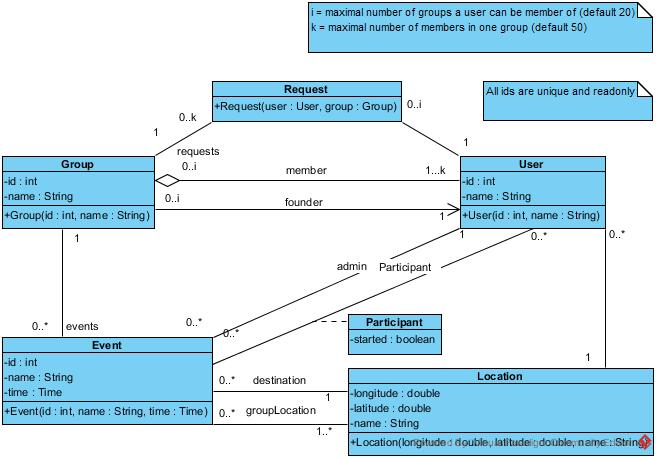
\includegraphics[width=0.9\paperwidth]{ModelClassDiagram.jpg}}
\end {center}
Ein Objektdiagramm zur Veranschaulichung des Modells mit Beispiel Objekten findet sich im \hyperlink{ModelExample}{Anhang}.

\newpage
	\subsubsection{DatabaseManagement}
	Die Klassen des DatabaseManagement sorgen für den Zugriff auf die Datenbank.
	Mittels Hibernate werden die gewünschten Daten aus der Datenbank abgerufen, geändert oder eingefügt und eine entsprechende Meldung an den Aufrufer gegeben.
	Dies ist unsere einzige Schnittstelle zur Datenbank.	
	\newline
Siehe Paketbeschreibung \hyperlink{database.management}{DatabaseManagement}.

\begin {center}
\makebox[0pt]{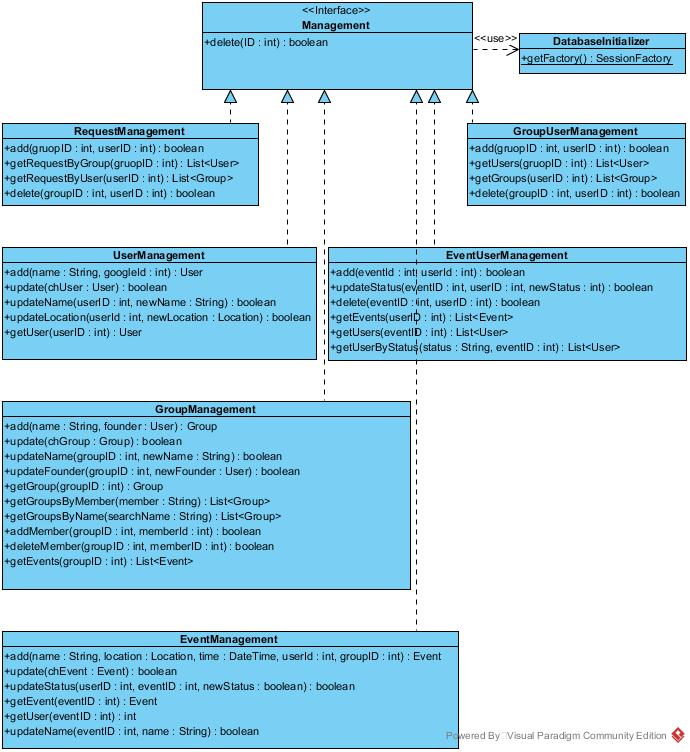
\includegraphics[width=0.92\paperwidth]{ManagementClassDiagram.jpg}}
\end {center}


	\subsubsection{Hibernate}
	Zur Verwaltung und Erstellung unserer Datenbank wollen wir das Hibernate-Framework nutzen. 
	Dies ermöglicht uns eine objektrelationale Abbildung, sodass wir unsere Java-Objekte in einer relationalen Datenbank speichern können und Beziehungen mit abgebildet werden.
	Ein großer Vorteil ist, dass die Datenbank von Hibernate erstellt und verwaltet wird, sodass spätere Änderungen im Modell einfach umgesetzt werden können.
	Wir nutzen das Hibernate-Framework, in dem wir in unseren Modell-Klassen für alle Klassen und Attribute Java-Annotations setzen.
	
	\subsubsection{Database}
	In der Datenbank werden für alle Elemente und Objekte die entsprechenden Daten gespeichert und bei Bedarf ausgelesen. Hierzu wird für jede Klasse des Modells sowie für bestimmte Beziehungen eine Tabelle angelegt.Identifiziert werden die jeweiligen Objekte durch eine eindeutige ID welche bei der Erstellung des Eintrags vergeben wird.Für Benutzer kommt diese ID von Google für die anderen Klassen wird die ID direkt von unserem Server vergeben.
	
\subsubsection{Clusteringalgorithmus}

Das Clusteralgorithmuspaket gruppiert Standorte und kann den Mittelpunkt mehrerer Standorte berechnen. Wir haben uns für das Entwurfsmuster Strategie entschieden, um die Implementierung der Clusteranalyse und Mittelpunktberechnung abzukapseln und austauschbar zu machen. Einzelne Klassen aus dem Clusteralgorithmuspaket sind in der Apache Commons Mathematics Bibliothek enthalten und müssen somit nicht mehr von uns implementiert werden. Wir verwenden Teile dieser Bibliothek, da sie unter der Apache License steht, gut getestet ist und perfekt zu unserem Projekt passt. Außerdem soll unser Projekt einen Mehrwert generieren und nicht darin bestehen vorhandene Software nachzubauen.\newline Das Clusteralgorithmuspaket kommuniziert direkt mit dem Paket DatabaseManagement und bekommt die Daten nicht von dem Servlet übergeben. Dies hat den Vorteil, dass die benötigten Daten nur von dem Algorithmus abhängig sind, was die Austauschbarkeit unterstützt. Neben den Klassen aus der Apache Bibliothek besteht dieses Paket aus einem eigenen Algorithmen zur Berechnung des Mittelpunkts bei der die Standorte unterschiedlich gewichtet werden, um einen möglichst sinnvollen Mittelpunkt zu erhalten. Da eine wichtige Funktionalität unserer App darin liegt, Standorte der Gruppe auf einer Karte anzeigen zu lassen, legen wir auch einen besonderen Wert auf eine sinnvolle Berechnung der Cluster.\newline
 Es gibt verschiedene Algorithmen, die an dieser Stelle sinnvoll sind, vor allem der DBSCAN-Algorithmus, bzw. der KMEANS-Algorithmus. Durch unsere Strategie können wir diese austauschen. Der DBSCAN-Algorithmus ist ein dichtebasierter Clusteralgorithmus und hat gegenüber dem KMEANS-Algorithmus den Vorteil, dass nicht vor der Berechnung klar sein muss wie viele Cluster entstehen sollen. Außerdem arbeitet er mit "Rauschen", bedeutet Punkte die keinem Cluster zugeordnet werden können, werden separat ausgegeben. Dabei arbeitet der Algorithmus mit einem Maximalabstand den Punkte zueinander haben dürfen. 
Der KMEANS-Algorithmus ist einer der meist genutzten Algorithmen zur Clusteranalyse und hat im Gegensatz zum DBSCAN-Algorithmus den Vorteil, dass er Cluster unterschiedlicher Dichte erkennen kann. Zudem bietet er ein signifikant besseres Laufzeitverhalten. Das Problem, dass in unserem Fall die Zahl der Cluster vor der Berechnung noch nicht feststeht, kann durch Evaluationsalgorithmen gelöst werden. Die Evaluationsalgorithmen werden in der Apache Bibliothek erst ab Version 4.0 angeboten, welche noch nicht offiziell veröffentlicht wurde, deren Clusterbibliothek jedoch schon gut getestet und online verfügbar ist.
Wir werden in der Implementierungsphase entscheiden ob wir die Apache Commons Math Bibliothek 4.0 oder 3.6.1 verwenden, da doch ein enormer Mehrwert durch die Version 4.0 entsteht.
\newline
Siehe Paketbeschreibung \hyperlink{algorithm}{Clusteringalgorithmus}.
  \newline
 
\begin {center}
\makebox[0pt]{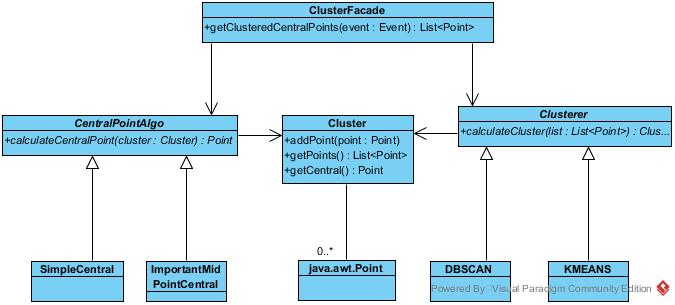
\includegraphics[width=0.95\paperwidth]{AlgorithmClassDiagram.jpg}}
\end {center}
\newpage
	\subsubsection{Servlets}

	Die Servlets nehmen die Anfragen der Clients entgegen. Diese ist ein JSON-String, welcher von den Servlets ausgelesen und danach entsprechend behandelt wird. Die Servlets leiten die erhaltenden Anfragen entweder an die Datenbankverwaltung oder an den Algorithmus weiter und schicken das Ergebnis an den Clienten.
Die Servlets fungieren als Schnittstelle zwischen den Anfragen des Clients und der eigentlichen Arbeit die auf dem Server vollbracht wird. 
Die Servlets sind in ihren Aufgabenbereichen unabhängig voneinander und auf das Modell angepasst, so gibt es z.B. ein Servlet, das alle Anfragen bezüglich eines Events beantwortet und ein weiteres, welches sich um die Handhabung der Gruppenbeitrittsanfragen kümmert.
Die Servlets sind auf die Services des Clients zugeschnitten, ein Servlet beantwortet also nur Anfragen von genau einem Service.
Für eine weitere Funktionalität kann also einfach ein neuer Service mit einem neuem Servlet unabhängig von allen anderen erstellt werden, was den Entwurf erweiterbar macht.   
\newline
Siehe Paketbeschreibung \hyperlink{servlet}{Servlets}.

\begin {center}
\makebox[0pt]{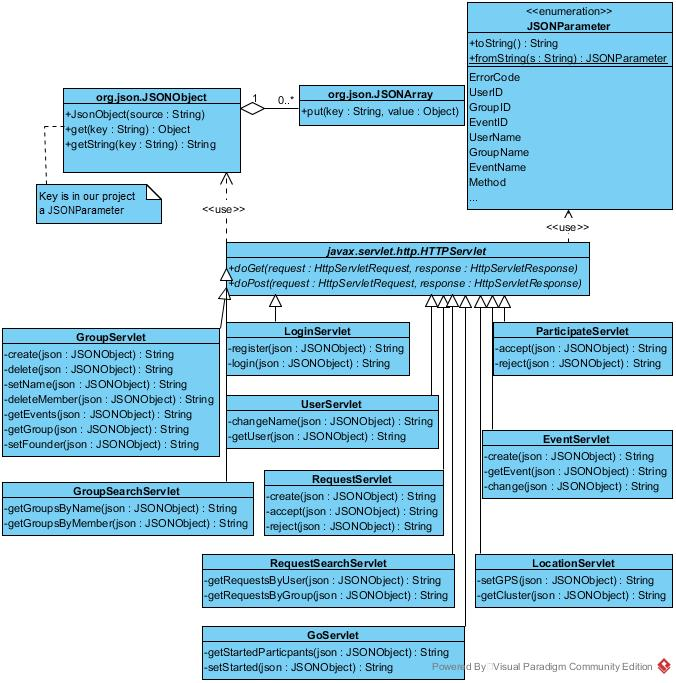
\includegraphics[width=0.95\paperwidth]{ServletsClassDiagram.jpg}}
\end {center}


	\subsection{Client}
	Auf den Clients ist die goApp installiert, sie wird eine Android-App sein, die dem Standard entsprechend in Java implementiert ist.
	Die goApp auf dem Client ist nach dem Muster Model-View-Controller aufgebaut. Damit wollen wir unseren Programmentwurf flexibel gestalten, was spätere Änderungen und Erweiterungen erleichtert. Außerdem erhöht diese Kapselung die Wiederverwendbarkeit der einzelnen Komponenten.
Sollte nachträglich noch eine iOS Version der goApp entstehen, lässt sich beispielsweise das Modell direkt übernehmen.
	
	\subsubsection{Services}
	Die Services sind der Controller des Clients und damit für die Steuerung zuständig. Hauptaufgabe ist es die Kommunikation zwischen der View und dem Server zu gewährleisten, aber auch Hintergrundprozesse anderer Art, wie das erstellen eines Timers, gehören in ihren Aufgabenbereich.
Sie sind, wie die Servlets, so entworfen, dass jeder Service seinen eigenen Aufgabenbereich übernimmt.
\newline Unsere Services erben alle von der Klasse IntentService woraus resultiert:
\begin{itemize}
\item sie laufen auf einen eigenem Thread
\item sie haben eine FIFO-Queue implementiert um mehrere Anfragen an den selben Service zu speichern und diese sequentiell abzuarbeiten
\item sie beenden sich automatisch wenn sie ihre Aufgabe erledigt haben
\end{itemize} 
\newpage
Von unserer App werden folgende Services implementiert:
\newline
\begin {center}
\makebox[0pt]{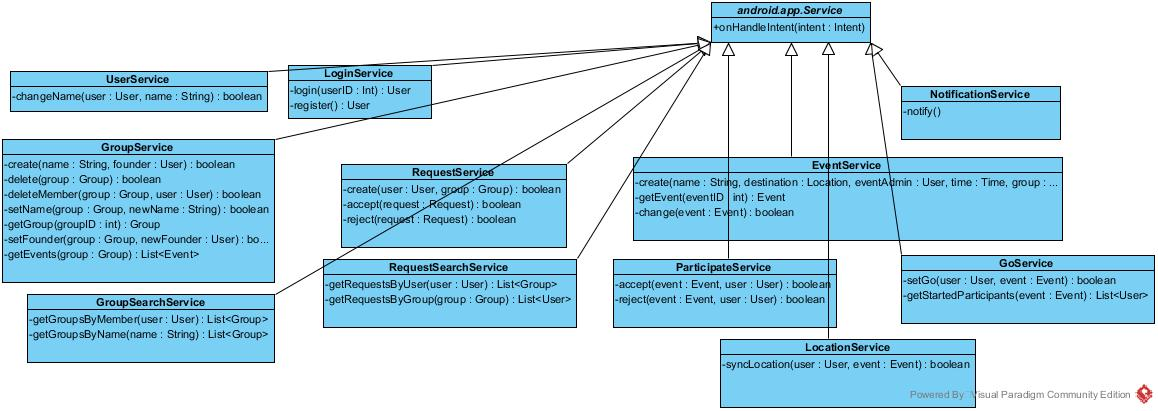
\includegraphics[width=0.9\paperwidth]{Controler.jpg}}
\end {center}
Siehe Paketbeschreibung \hyperlink{controler.service}{Services}.
\newpage
	\subsubsection{Activities}
Alle Activities setzten sich aus aus einer Java Klasse für die Logik, sowie einer XML-Datei für das Design der View zusammen. Eine Activity kann mehrere Fragments enthalten.
Sie nehmen als erstes Benutzerinteraktionen entgegen, leiten diese an den entsprechenden Service weiter und geben dem User entsprechendes Feedback.
\newline Eine Activity kann in unserer App drei Zustände haben:
\begin{itemize}
\item Sie ist aktiv, läuft im Vordergrund und wird dem Benutzer angezeigt.
\item Sie ist gestoppt durch den Wechsel auf eine andere Activity. Auch wenn der Benutzer sie in diesem Zustand nicht sehen kann, behält sie ihren aktuellen Status und muss deshalb nicht neu geladen werden falls man zu ihr zurück navigiert.
\item Sie ist beendet durch das Betriebssystem.  Um die Activity dann wieder anzuzeigen muss sie neu gestartet werden und Daten müssen erneut geladen werden.
\end{itemize}
\newpage
Eine Activity hat folgenden Lebenszyklus:\newline
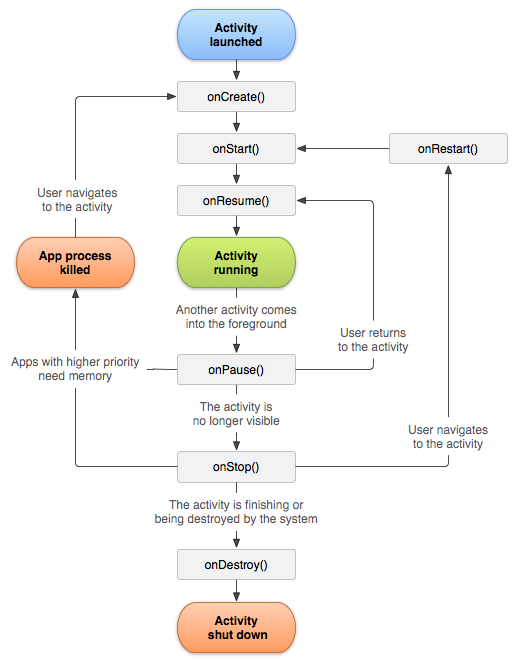
\includegraphics[width=.9\textwidth]{activity_lifecycle.png}
\textit{\newline Quelle: https://developer.android.com/reference/android/app/Activity.html}
\newpage
Unsere App besitzt folgende Activities:
\newline

\begin {center}
\makebox[0pt]{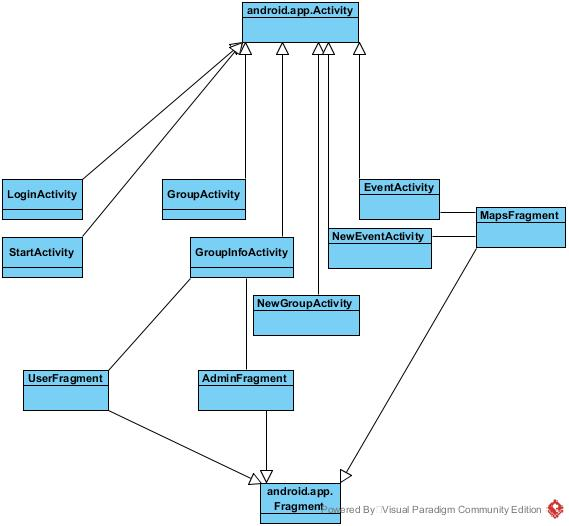
\includegraphics[width=0.9\paperwidth]{ViewClassDiagram.jpg}}
\end {center}

Siehe Paketbeschreibung \hyperlink{view}{Activities}.
	\newpage
	\subsubsection{Modell}
Das Modell versucht die Realität auf die Daten des Servers und der Applikation abzubilden und ist von dem Controller und der View unabhängig. 
Das Modell auf dem Client entspricht dem Modell des Servers.

	\subsubsection{ServerConnection}
	Die Klasse HTTPConnection bildet die Schnittstelle zwischen dem Server und dem Client. Die Services schicken Anfragen an sie. Diese werden über eine HTTP-Verbindung an die entsprechenden Servlets des Servers weitergeleitet und deren Antwort gibt HTTPConnection wieder an den Service zurück.
\newline
Siehe Paketbeschreibung \hyperlink{controler.serverConnection}{ServerConnection}.

\begin {center}
\makebox[0pt]{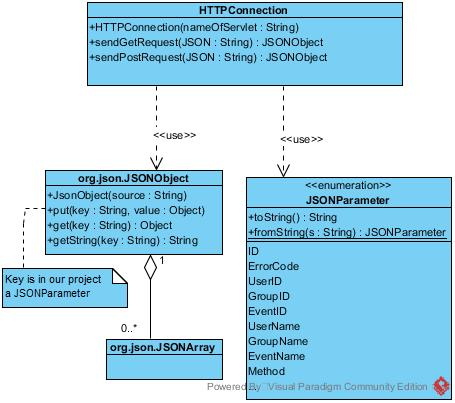
\includegraphics[width=0.95\textwidth]{HTTPClientClassDiagram.jpg}}
\end {center}
\newpage
	\subsection{Fehlerbehandlung}
Wenn auf dem Server ein Fehler auftritt wird dieser vom Servlet abgefangen und in dem JSON-String der Antwort eingetragen. Dafür gibt es einen ErrorCode Parameter in der Klasse JSONParameter. Durch diesen Fehlercode in der Serverantwort wird dem Client der Fehler mitgeteilt.\par

Da auf dem Client keine wichtigen Daten gespeichert sind werden hier die auftretenden Fehler nur an den Benutzer mit einer aussagekräftigen Meldung weiter gegeben. Außerdem werden alle Informationen atomar übergeben und können zusätzlich noch neu vom Server geladen bzw. an den Server geschickt werden. \par

Unsere Kommunikation beinhaltet keine kritischen Daten, die explizit nur einmal gesendet werden sollen. Dadurch werden keine zustandssichernden Maßnahmen benötigt, um auf den Zustand vor dem Fehler zurückkehren zu können und z.B. gescheiterte Anfragen neu zu stellen.

	\newpage
